\chapter{Prologue}\label{chap:intro}
\openepigraph{\emph{Echoes} shows the direction that we’re moving in.}{David Gilmour,\\ making of ``The Dark Side Of The Moon''}
% \openepigraph{One does not simply [...]}{Boromir}

\vspace{-2.5em}
% \marginpar{%
%     \footnotesize
%     \textbf{Resources:}
%     \begin{itemize}
%         \item[\faYoutube] \href{https://www.youtube.com/watch?v=lLUcOFwZvyY&t=22s}{Testing The World's Longest Echo}
%         \item[\faYoutube] \href{https://www.youtube.com/watch?v=px3oVGXr4mo}{SKUNK BEAR : What Does Sound Look Like?}
%         \item[\faYoutube] \href{https://www.youtube.com/watch?v=ZwgovJSQ5UM}{ARTE : La Magie Du Son}
%         \item[\faYoutube] \href{https://www.youtube.com/watch?v=uH0aihGWB8U&t=631s}{Daniel Kish: How I use sonar to navigate the world}
%     \end{itemize}
% }


\def\MyText{\textsc{Echoooes}}
\newcommand\mytext[2][black]{\scalebox{#2}{\textcolor{#1}{\MyText}}}

\newthought{In a nutshell,} this \PhD/ thesis is about acoustic
\stackinset{c}{4ex}{c}{ 1.4ex}{\mytext[black!70]{.8}}{%
\stackinset{c}{2ex}{c}{ 3.2ex}{\mytext[black!25]{.7}}{%
\stackinset{c}{3ex}{c}{-1.3ex}{\mytext[black!35]{.9}}{%
\mytext{1}%
}}}.
\\We live immersed in a complex acoustical world, where every concrete thing can sound, resound, and echo.
For humans, it is difficult to internalize what is sound, its constituents, and its generation.
It is processed by our auditory system and brain so efficiently that our attention is detached from the physical laws governing it.
Therefore, when listening to something, we typically focus directly on its \textit{semantic content}.
Evolution lead us to conduct this process without any efforts, despite the presence of a high level of background noise, for instance during a concert.
This outstanding capability is not limited to humans and is common to many of the creatures we are sharing the physical world with.

% When we listen to music, we focus on the melody in the music; when listen to speech, we focus on the words;
% \\However not only \textit{semantic information} about the source is carried by the sound.
% There are many other types of information that we retrieve and infer from it, such as \textit{temporal} and \textit{spatial} information.
% For instance, we are able to localize its source:
% if someone is calling us, we unconsciously know towards where to turn.
% We can guess if an noisy motorbike is approaching or moving away.
% Another striking example, which involves simple math, is estimating of how far the storm is, simply counting the time between a view a lightning a listening to thunder.
% We can even guess the size and the type of the room we are currently sitting in.

\mynewline
Nonetheless, we process many other information of the complex \textit{acoustic scenes} we are immersed into.
In addition to the semantic content, a sound also conveys \textit{temporal} and \textit{spatial} information.
For instance, the ticking of a metronome\sidenote{
    For his experiments, Galileo Galilei was measuring time using the sound of a metronome.
} or clock provides units of time and when hearing someone shouting, we unconsciously know where to turn our attention.
% Therefore, as for the content, this information is still carried by the sound.
However, this information is determined by how sound \textit{propagates} in space and not by the source itself.

\mynewline
Before reaching the ears, sound propagates in all directions and a portion of its energy arrives at us directly, and another indirectly, after being reflected around.
This process leads to the creation of \textit{echoes} and \textit{reverberation}.
Typical examples are the echoes produced by large rocky mountains or walls in monumental buildings, such as the Panthéon in Rome or the Pont de Neuilly in Paris.
\sidenote{
    ``\textit{Écho. Citer ceux du Panthéon et du pont de Neuilly.}''
    --- Gustave Flaubert, \textit{Dictionnaire des idées reçues}.
}
In common language, echoes refer to distinctive reflected sounds which can be heard, thus, characterized by a specific \textit{time of arrival} and \textit{attenuation}.
In smaller environments, echoes are still present but are typically less perceived as they arrive more quickly and densely.
What is perceived here is the so-called reverberation, for which large empty rooms or churches are great examples.

\mynewline
Some animals evolved to ``see'' thanks to echoes.
Two of the most striking examples are bats and whales which use them for navigation and hunting.
By emitting sound patterns and listening to their reflections returned from the environment, these animals scan the surrounding space, identifying and locating objects.
Here, the echoes are voluntarily produced and this is referred to as \textit{active echo-location} or (bio) sonar.
In contrast, in \textit{passive} echo-location, external, unknown sound sources are used instead.
\marginpar{
    \footnotesize
    \itshape
    This technique is developed instinctively by some blind people as well.
    By tapping their canes or clicking their tongues, they are able for instance to avoid obstacles when walking.
    In the 18th century, French philosopher Denis Diderot recorded the this incredible ability, which was labeled as ``echo-location'' only 300 years later by Donald Griffin.
    ~\citeonly{kolarik2014summary}.
}
``Locating it'' means estimating its delay with respect to the direct sound.
These delays are then processed as distances in the brain, in the same way our grandparents taught us to localize a storm by counting the time between a lightning and its thunder.
That is how bats and whales find preys, see obstacles, and orientate themselves in dark caves or deep seas.
However, the term ``echo-location'' here could be misleading as it may solely refer to the to the only problem of locating objects.
As we will discuss later, the application of echoes goes beyond simple localization.
Therefore, in this thesis, we will prefer the terminology of \textit{echo estimation}.

\mynewline
Remarkable examples of passive echo estimation in nature are not very well known.
Sand scorpions use the propagation of vibrations in the sand to follow the movement of other insects in the dark night.
By using their 8 legs as a radar, they perform passive (seismic) echo-location with inevitable consequences for the prey.
This technique is common to spiders who sense reverberation in their complex web\sidenote{
    According to some recent studies, spiders appear to offload cognitive tasks to their webs.
    The web may then act then as a complex system processing and filtering the information, which is then returned to their owner.
    \citeonly{sokol2017thoughts}
}.
They are not only able to localize the preys fast, but also to identify them, and disambiguate them from simple objects moved by the wind or malicious visitors.
In this case, instead of emitting sounds, evolution taught them to use complex structures (for scorpions their legs, for spiders webs) in order to feed and survive.

\mynewline
Echoes do not only serve for computing distances or localizing preys.
For instance, they make speech more intelligible, improve our sense of orientation and balancing\citeonly[Chapter 5.4]{huggett1953human}, and provide music with ``dimensionality''\citeonly{sacks2014musicofilia}.
This phenomenon is a branch of study in \textit{room acoustics}, \textit{pyschoacoustics} and \textit{sound design}.
In particular, the former study acoustic echoes for designing theatres, auditoriums and meeting rooms, with the aim of a good listening quality.

\mynewline
% To conclude with, this thesis focuses on how to estimate passively acoustic echoes and how to used them to achieve better audio analysis.
% This investigation is conducted in the context of indoor audio signal processing.
The problems addressed in this thesis are indicated in the thesis title: \textit{Echo-aware signal processing for audio scene analysis}.
There are three parts in the sentence that deserve an explanation: \textit{echo-aware}, \textit{signal processing} and \textit{audio scene analysis}.
In order, we will first elaborate the last two as they contextualize this thesis, and after, we will explain why and how echoes help.

% \mynewline
% One may ask, what does it mean, to estimate echoes and use them?
% Therefore with echo estimation we will refer to the estimation of them both.
% Even there are less clear example in nature to explain it, passive echo location is used by our mind instinctively in order to process the acoustic scene.
% Therefore, in the context of computer science, it is natural to ask ourself how we can build machine that can listen as we do?
% How is it implemented? it will be outlined in the next section.

\section{Audio signal processing}\label{sec:intro:processing}
% In order to process sounds, machines and computer use algorithmic tools which fall in the research field of \textit{audio signal processing}.
\textit{Signal processing} is the process of analyzing and modifying a \textit{signals}, which are mathematical representations of quantities carrying information about a phenomenon.
In \textit{audio signal processing}, this phenomenon is sound.
Typical signals are speech or music, and various mathematical and algorithmic techniques have been developed to process them.
\marginpar{
    \footnotesize
    \textit{Audio is a used as a technical term, referring to sound coming from a recording and transmission.
    Acoustic, instead, refer to the physical aspect of sound.}
}
There are multiple reasons to do this, such as producing new signals with higher quality or and retrieving high-level information that the signal carry.
To this end, complex systems are built which can be represented as a collection of simpler subsystems, with well-defined tasks, interacting with each other.
In (audio) signal processing, these subsystems roughly fall into four categories: \textit{representation}, \textit{enhancement}, \textit{estimation}, and \textit{adaptive processing}.
Many related problems can be then decomposed into blocks which are include one or more of the following steps.

\newthought{Representation}.
    The signals can be represented in many different ways, so that the \textit{information} they contain becomes more easily accessible for specific tasks.
    It is generally implemented through \textit{change of domain} or \textit{feature extraction}.
    In audio, the most widely used representation is the Fourier basis, which changes the signal domain from time to frequencies.

\newthought{Enhancement}.
    Observed signals may be affected by distortions, which corrupts and hides the relevant information.
    Examples of these are measurement and quantization noise, noisy sources, reverberation, clipping, \etc/.
    Therefore, signal enhancement, namely, reducing any form of distortion, is typically a necessary step.
    Practical examples of enhancement are removing background noise from a mobile phone recording, isolating instrument tracks from in a song, \etc/.

\newthought{Estimation}.
    Often, we wish to estimate some key properties of the target signal, which may be used as inputs to a different algorithm.
    For instance, we may be interested in estimating a speaker's position in a recording, the time of arrival of an echo, or the pitch of a sound.

\newthought{Adaptive processing}.
    It deals with algorithms that are able to adapt themselves to the data.
    They typically process the data on the fly and are controlled by variable parameters resulting from previous estimation blocks.
    They usually rely on the optimization of an objective function designed to meet specific requirements.
    Examples of these algorithms are present in noise-canceling headphones or echo cancellation modules implemented in video conference call systems.



\section{Audio scene analysis}\label{sec:intro:scene}
Pay attention to what you are hearing right now:
there might be music, someone talking to you, footsteps echoing in the other room, background noise due to cars, a heating system, maybe rain or wind, the sound of your movements, and many others.
Everything you hear now as well as its location in space is what is called the \textit{audio scene}\sidenote{
    The correct terminology for it is \textit{auditory scene}, which relates to human perception.
    Psychologist Albert Bregman in~\citeonly{bregman1990auditory} coined it.
    However, we will use this terminology since we extend this concept to audio signal processing, and as it is commonly accepted in the literature.
}.
Therefore, \textit{audio scene analysis} is trivially the analysis of it\marginpar{
    \footnotesize\itshape
    From the ancient greek, \emph{analysis} means dismantling into constituent elements.
    It allows then to reach information otherwise obfuscated by the big picture.
    It is opposed to \emph{synthesis}, which instead combines parts into a whole.
}.
More specifically, the extraction and organization of all the information contained in the sound associated with an audio scene.

\mynewline
In audio signal processing, this process involves using algorithmic and mathematical tools to retrieve and organize such information.
% \marginpar{
%     \footnotesize\itshape
%     Thinking of the technologies behind Google Home and Amazon Alexa, one may wonder the ethical implication of audio scene analysis.
%     During this thesis's work, these issues have resulted in discussions with colleagues and friends, but it will be discussed in another forum.
%     \href{https://techcrunch.com/2016/12/27/an-amazon-echo-may-be-the-key-to-solving-a-murder-case/}{Amazon Echo\ExternalLink}
% }
After recording the audio scene with microphones, complex systems, as described above, are used to access the information.
Accessing different types of information at different levels of complexity leads to the definition of different \textit{problems}.
These problems focus on well-defined tasks and some are referred to with established names.
\cref{tab:processing:problems} lists some selected audio scene analysis problems that will be considered later in this thesis.

\begin{table}[!h]

    \begin{fullwidth}
    \centering
    \small

    \begin{tabular}{p{0.33\linewidth} p{0.66\linewidth}}
    \toprule
    Problems & \textit{From the recordings, can we...} \\
    \midrule
    Audio Source Separation   & ... estimate the audio signal of sound sources?\\

    Audio Source Enhancement   & ... estimate the audio signal of a target sound source?\\

    Sound Source Localization & ... estimate the positions of sounds sources? \\

    Microphone Calibration    & ... positions and properties of the microphones?? \\

    Room Geometry Estimation  & ... estimate the shape of the room? \\

    Acoustic Echo Estimation  & ... estimate the echoes' properties? \\

    Acoustic measurement      & ... estimate physical properties related to sound propagation?\\

    \hline
    Source Identification     & ... estimated the type of source signal?\\

    Speech Diarization        & ... who is speaking and when ? \\

    Source Counting           & ... count the number of speaker s? \\

    Automatic Speech Recordings & ... the content of the speech ? \\

    \bottomrule
\end{tabular}
    \caption{List of selected audio scene analysis problems. The one above the line are considered in this thesis.}
    \label{tab:processing:problems}

    \end{fullwidth}

\end{table}

\mynewline
Without getting too philosophical, it is possible to re-cast these problems to some (simple) human interrogations:
\begin{itemize}
    \item  \textit{What?} Answered by Audio Source Separation and Enhancement, Automatic Speech Recognition, and Source Identification, operating on the source signals' semantic content;
    \item  \textit{Where?} Answered by Sound Source Localization, Microphone Calibration, and Room Geometry Estimation, by elaborating the spatial information of the sound propagation;
    \item  \textit{When?} Answered by Speech Diarization, or leveraging the sound temporal information;
\end{itemize}

\noindent Our\openepigraph{Everything is connected}{Douglas Adams, \textit{Dirk Gently's Holistic Detective Agency}}
brain and the auditory system can instantly and often effortlessly solve these problems, such that they may seem like trivial tasks.
However, they hide many difficult challenges when it comes to designing efficient and robust algorithms.
Moreover, most of these problems may exhibit strong inter-connections, and the solution of one of them depends on the solution of others.
For instance, knowing when someone is speaking and its location in the room, sound source separation can be achieved more easily.
This should not be surprising since it bears a strong parallelism with our everyday experience.

\mynewline
Similarly, echoes may help audio signal processing.

\section{The echo-aware approach}
As proven by natural behaviors, acoustic echoes are important for humans and animals to analyze the audio scene:
As repetitions of a sound, they convey information about that sound.
As characterized by temporal instants and attenuation related to distances, they convey spatial information about the audio scene.
As modified by the frequency description of the object that generates them, they convey acoustic information about it.
\\This observation motivated many researchers to include echoes in signal processing applications, not only limited to audio\sidenote{
    The idea of integrating reflection in models is also studied in other fields of engineering.
    In telecommunication and networking, for instance, where these phenomena are referred to as \textit{multipath propagation}.
}.
However, it was not always the case.
Many audio scene analysis methods make limiting assumptions on of the sound propagation to derive efficient algorithms.
One of the most common ones is the so-called \textit{anechoic} or \textit{free-field} scenario, assuming neither echoes nor reverberation is present in the audio scene.
Even if this assumption can be seen as reasonable in some scenarios, it is easy to understand its underlying limitations when applied to real-world recordings.
Furthermore, in some cases, echoes are considered a source of noise and interference and then modeled as something to cancel out.

\mynewline
Instead, some researchers proposed to explicitly include acoustic echoes in leading to what we will refer to as \textit{echo-aware methods}.
Some of the earliest examples in this direction are the works of Flanagan et al\citeonly{flanagan1993spatially, jan1995matched, jan1996sound} in source enhancement.
However, only recently, these methods have regained interest in audio processing as manifested by the European project SCENIC~\citeonly{Annibale2011scenic} and the UK research \href{http://www.s3a-spatialaudio.org/}{S$^3$A project}.
In some recent studies, echoes are used to boost performances of typical audio scene analysis problems, \eg/, speech enhancement \citeonly{Dockmanic2015raking, Kowalczyk2019raking}, sound source localization \citeonly{ribeiro2010turning}, and source separation \citeonly{scheibler2017separake, leglaive2016multichannel, remaggi2019modeling}, and room geometry estimation from sound \citeonly{remaggi2016acoustic, dokmanic2013acoustic, crocco2017uncalibrated}.

\mynewline
All these methods show the importance and the benefits of modeling acoustic reflections.
However, prior to all of them is the \AERdef/ problem.
This step, which is most often given for granted in the above applications, is extremely challenging, as shown throughout this entire thesis work.

\section{Thesis outline and main contributions}
The\openepigraph{Sometimes a scream is better than a thesis.}{Ralph Waldo Emerson} goal of this thesis is to improve the current state-of-the-art for indoor audio signal processing along two axes:
\begin{enumerate}
    \item Provide new methodologies and data to process and estimate acoustic echoes and surpass the limits of current approaches.
    \item Extend previous classical methods for audio scene analysis by incorporating the knowledge of echo properties in sound propagation models.
\end{enumerate}
These two goals are elaborated in the two main parts of the thesis, which follow after an introductory one, as summarized below.
However the parts are largely interconnected, as shown in~\cref{fig:intro:thesis_mindmap}.

\begin{figure}[t]
    \begin{sidecaption}[Thesis Organization]{%
        Schematic organization of the thesis, dependencies between chapters linked to author contributions.
    }[fig:intro:thesis_mindmap]
    \centering
    \resizebox{\linewidth}{!}{
        

\tikzset{every picture/.style={line width=0.75pt}} %set default line width to 0.75pt

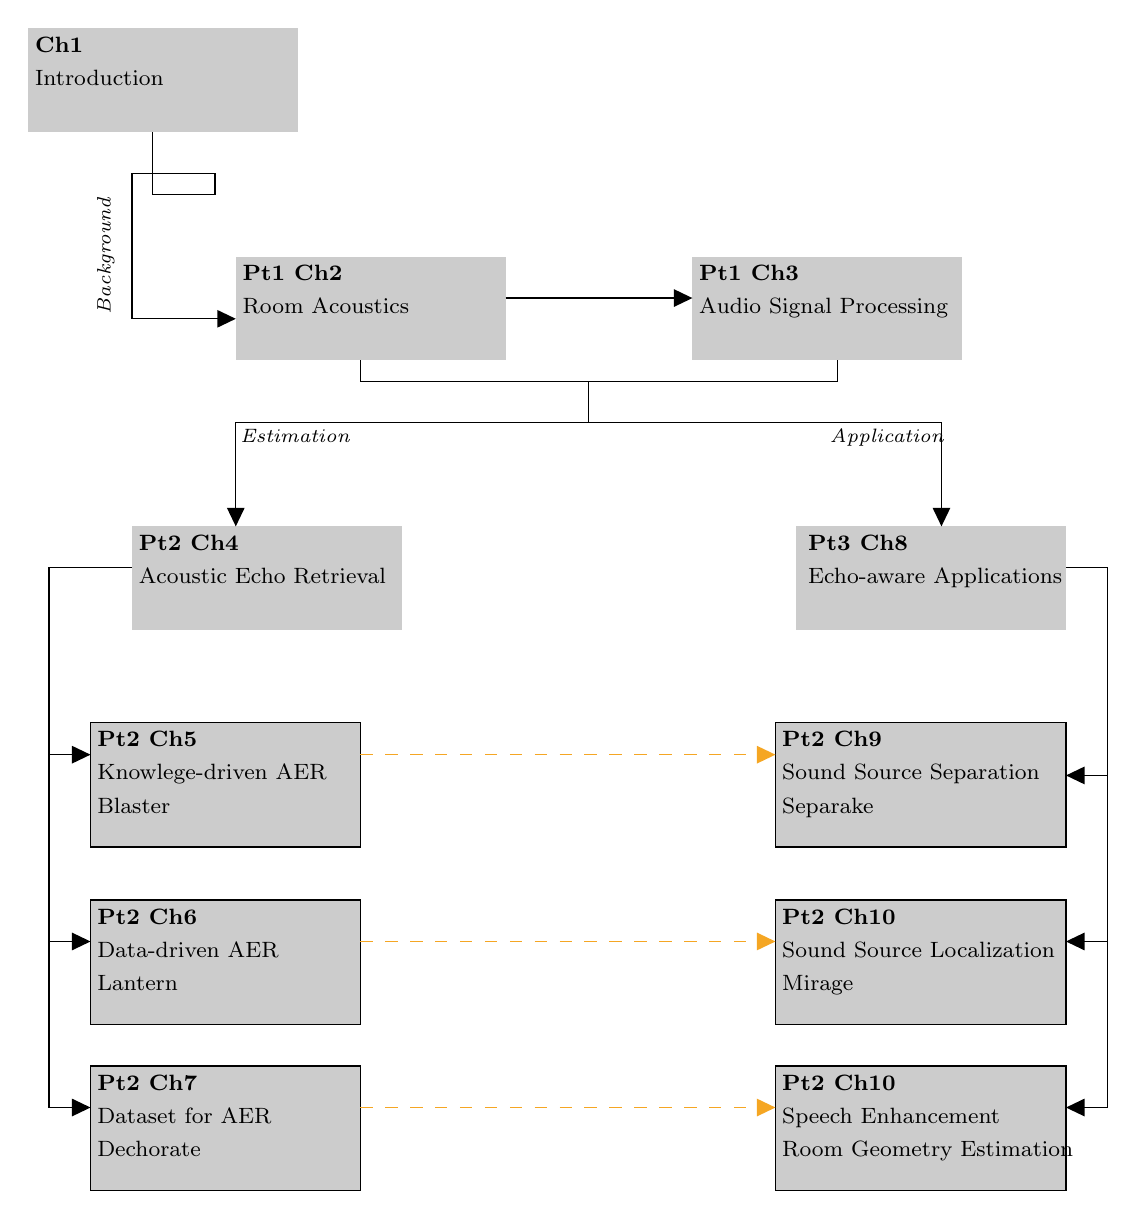
\begin{tikzpicture}[x=0.75pt,y=0.75pt,yscale=-1,xscale=1]
%uncomment if require: \path (0,621); %set diagram left start at 0, and has height of 621

%Shape: Rectangle [id:dp5066015063615144]
\draw  [draw opacity=0][fill={rgb, 255:red, 0; green, 0; blue, 0 }  ,fill opacity=0.2 ] (130,130) -- (260,130) -- (260,180) -- (130,180) -- cycle ;
%Shape: Rectangle [id:dp5704675358971985]
\draw  [draw opacity=0][fill={rgb, 255:red, 0; green, 0; blue, 0 }  ,fill opacity=0.2 ] (350,130) -- (480,130) -- (480,180) -- (350,180) -- cycle ;
%Shape: Rectangle [id:dp4921892891726769]
\draw  [draw opacity=0][fill={rgb, 255:red, 0; green, 0; blue, 0 }  ,fill opacity=0.2 ] (30,20) -- (160,20) -- (160,70) -- (30,70) -- cycle ;
%Shape: Rectangle [id:dp2703924787206532]
\draw  [draw opacity=0][fill={rgb, 255:red, 0; green, 0; blue, 0 }  ,fill opacity=0.2 ] (80,260) -- (210,260) -- (210,310) -- (80,310) -- cycle ;

%Shape: Rectangle [id:dp16360886559522403]
\draw  [color={rgb, 255:red, 0; green, 0; blue, 0 }  ,draw opacity=1 ][fill={rgb, 255:red, 0; green, 0; blue, 0 }  ,fill opacity=0.2 ] (60,354.5) -- (190,354.5) -- (190,414.5) -- (60,414.5) -- cycle ;

%Shape: Rectangle [id:dp3170404537266921]
\draw  [color={rgb, 255:red, 0; green, 0; blue, 0 }  ,draw opacity=1 ][fill={rgb, 255:red, 0; green, 0; blue, 0 }  ,fill opacity=0.2 ] (60,440) -- (190,440) -- (190,500) -- (60,500) -- cycle ;

%Shape: Rectangle [id:dp34273699987381434]
\draw  [color={rgb, 255:red, 0; green, 0; blue, 0 }  ,draw opacity=1 ][fill={rgb, 255:red, 0; green, 0; blue, 0 }  ,fill opacity=0.2 ] (60,520) -- (190,520) -- (190,580) -- (60,580) -- cycle ;

%Shape: Rectangle [id:dp40314291935103563]
\draw  [draw opacity=0][fill={rgb, 255:red, 0; green, 0; blue, 0 }  ,fill opacity=0.2 ] (400,260) -- (530,260) -- (530,310) -- (400,310) -- cycle ;

%Shape: Rectangle [id:dp7794772177604954]
\draw  [color={rgb, 255:red, 0; green, 0; blue, 0 }  ,draw opacity=1 ][fill={rgb, 255:red, 0; green, 0; blue, 0 }  ,fill opacity=0.2 ] (390,354.5) -- (530,354.5) -- (530,414.5) -- (390,414.5) -- cycle ;

%Shape: Rectangle [id:dp34646122412068336]
\draw  [color={rgb, 255:red, 0; green, 0; blue, 0 }  ,draw opacity=1 ][fill={rgb, 255:red, 0; green, 0; blue, 0 }  ,fill opacity=0.2 ] (390,440) -- (530,440) -- (530,500) -- (390,500) -- cycle ;

%Shape: Rectangle [id:dp3115018720256666]
\draw  [color={rgb, 255:red, 0; green, 0; blue, 0 }  ,draw opacity=1 ][fill={rgb, 255:red, 0; green, 0; blue, 0 }  ,fill opacity=0.2 ] (390,520) -- (530,520) -- (530,580) -- (390,580) -- cycle ;
%Straight Lines [id:da9308319505671777]
\draw    (90,70) -- (90,100) -- (120,100) -- (120,90) -- (80,90) -- (80,160) -- (127,160) ;
\draw [shift={(130,160)}, rotate = 180] [fill={rgb, 255:red, 0; green, 0; blue, 0 }  ][line width=0.08]  [draw opacity=0] (8.93,-4.29) -- (0,0) -- (8.93,4.29) -- cycle    ;
%Straight Lines [id:da047091716352255064]
\draw    (260,150) -- (347,150) ;
\draw [shift={(350,150)}, rotate = 180] [fill={rgb, 255:red, 0; green, 0; blue, 0 }  ][line width=0.08]  [draw opacity=0] (8.93,-4.29) -- (0,0) -- (8.93,4.29) -- cycle    ;
%Straight Lines [id:da70649725907847]
\draw    (190,180) -- (190,190) -- (300,190) -- (300,210) -- (130,210) -- (130,257) ;
\draw [shift={(130,260)}, rotate = 270] [fill={rgb, 255:red, 0; green, 0; blue, 0 }  ][line width=0.08]  [draw opacity=0] (8.93,-4.29) -- (0,0) -- (8.93,4.29) -- cycle    ;
%Straight Lines [id:da8610022387933317]
\draw    (300,210) -- (470,210) -- (470,257) ;
\draw [shift={(470,260)}, rotate = 270] [fill={rgb, 255:red, 0; green, 0; blue, 0 }  ][line width=0.08]  [draw opacity=0] (8.93,-4.29) -- (0,0) -- (8.93,4.29) -- cycle    ;
%Straight Lines [id:da5888330434056945]
\draw    (80,280) -- (40,280) -- (40,370) -- (57,370) ;
\draw [shift={(60,370)}, rotate = 180] [fill={rgb, 255:red, 0; green, 0; blue, 0 }  ][line width=0.08]  [draw opacity=0] (8.93,-4.29) -- (0,0) -- (8.93,4.29) -- cycle    ;
%Straight Lines [id:da40423722405051754]
\draw    (40,370) -- (40,460) -- (57,460) ;
\draw [shift={(60,460)}, rotate = 180] [fill={rgb, 255:red, 0; green, 0; blue, 0 }  ][line width=0.08]  [draw opacity=0] (8.93,-4.29) -- (0,0) -- (8.93,4.29) -- cycle    ;
%Straight Lines [id:da17759111494744462]
\draw    (40,460) -- (40,540) -- (57,540) ;
\draw [shift={(60,540)}, rotate = 180] [fill={rgb, 255:red, 0; green, 0; blue, 0 }  ][line width=0.08]  [draw opacity=0] (8.93,-4.29) -- (0,0) -- (8.93,4.29) -- cycle    ;
%Straight Lines [id:da6275082485537149]
\draw    (530,280) -- (550,280) -- (550,380) -- (533,380) ;
\draw [shift={(530,380)}, rotate = 360] [fill={rgb, 255:red, 0; green, 0; blue, 0 }  ][line width=0.08]  [draw opacity=0] (8.93,-4.29) -- (0,0) -- (8.93,4.29) -- cycle    ;
%Straight Lines [id:da22068584313938533]
\draw    (550,380) -- (550,460) -- (533,460) ;
\draw [shift={(530,460)}, rotate = 360] [fill={rgb, 255:red, 0; green, 0; blue, 0 }  ][line width=0.08]  [draw opacity=0] (8.93,-4.29) -- (0,0) -- (8.93,4.29) -- cycle    ;
%Straight Lines [id:da8344737228139845]
\draw    (550,460) -- (550,540) -- (533,540) ;
\draw [shift={(530,540)}, rotate = 360] [fill={rgb, 255:red, 0; green, 0; blue, 0 }  ][line width=0.08]  [draw opacity=0] (8.93,-4.29) -- (0,0) -- (8.93,4.29) -- cycle    ;
%Straight Lines [id:da9035501913545279]
\draw [color={rgb, 255:red, 245; green, 166; blue, 35 }  ,draw opacity=1 ] [dash pattern={on 4.5pt off 4.5pt}]  (190,370) -- (387,370) ;
\draw [shift={(390,370)}, rotate = 180] [fill={rgb, 255:red, 245; green, 166; blue, 35 }  ,fill opacity=1 ][line width=0.08]  [draw opacity=0] (8.93,-4.29) -- (0,0) -- (8.93,4.29) -- cycle    ;
%Straight Lines [id:da9667162690545281]
\draw [color={rgb, 255:red, 245; green, 166; blue, 35 }  ,draw opacity=1 ] [dash pattern={on 4.5pt off 4.5pt}]  (190,460) -- (387,460) ;
\draw [shift={(390,460)}, rotate = 180] [fill={rgb, 255:red, 245; green, 166; blue, 35 }  ,fill opacity=1 ][line width=0.08]  [draw opacity=0] (8.93,-4.29) -- (0,0) -- (8.93,4.29) -- cycle    ;
%Straight Lines [id:da45489191440409493]
\draw [color={rgb, 255:red, 245; green, 166; blue, 35 }  ,draw opacity=1 ] [dash pattern={on 4.5pt off 4.5pt}]  (190,540) -- (387,540) ;
\draw [shift={(390,540)}, rotate = 180] [fill={rgb, 255:red, 245; green, 166; blue, 35 }  ,fill opacity=1 ][line width=0.08]  [draw opacity=0] (8.93,-4.29) -- (0,0) -- (8.93,4.29) -- cycle    ;
%Straight Lines [id:da3297497661384694]
\draw    (300,190) -- (420,190) -- (420,180) ;

% Text Node
\draw (132,133) node [anchor=north west][inner sep=0.75pt]   [align=left] {\textbf{{\footnotesize Pt1 Ch2}}\\{\footnotesize Room Acoustics}};
% Text Node
\draw (32,23) node [anchor=north west][inner sep=0.75pt]   [align=left] {\textbf{{\footnotesize Ch1}}\\{\footnotesize Introduction}};
% Text Node
\draw (404.5,263) node [anchor=north west][inner sep=0.75pt]   [align=left] {\textbf{{\footnotesize Pt3 Ch8}}\\{\footnotesize Echo-aware Applications}};
% Text Node
\draw (392,357.5) node [anchor=north west][inner sep=0.75pt]   [align=left] {\textbf{{\footnotesize Pt2 Ch9}}\\{\footnotesize Sound Source Separation}\\{\footnotesize \library{Separake}}};
% Text Node
\draw (62,357.5) node [anchor=north west][inner sep=0.75pt]   [align=left] {\textbf{{\footnotesize Pt2 Ch5}}\\{\footnotesize Knowlege-driven \ac{AER}}\\{\footnotesize \library{Blaster}}};
% Text Node
\draw (392,443) node [anchor=north west][inner sep=0.75pt]   [align=left] {\textbf{{\footnotesize Pt2 Ch10}}\\{\footnotesize Sound Source Localization}\\{\footnotesize \library{Mirage}}};
% Text Node
\draw (62,443) node [anchor=north west][inner sep=0.75pt]   [align=left] {\textbf{{\footnotesize Pt2 Ch6}}\\{\footnotesize Data-driven \ac{AER}}\\{\footnotesize \library{Lantern}}};
% Text Node
\draw (62,523) node [anchor=north west][inner sep=0.75pt]   [align=left] {\textbf{{\footnotesize Pt2 Ch7}}\\{\footnotesize Dataset for \ac{AER}}\\{\footnotesize \library{Dechorate}}};
% Text Node
\draw (131,212) node [anchor=north west][inner sep=0.75pt]   [align=left] {{\scriptsize \textit{Estimation}}};
% Text Node
\draw (415,212) node [anchor=north west][inner sep=0.75pt]   [align=left] {{\scriptsize \textit{Application}}};
% Text Node
\draw (62,159) node [anchor=north west][inner sep=0.75pt]  [rotate=-270] [align=left] {{\scriptsize \textit{Background}}};
% Text Node
\draw (82,263) node [anchor=north west][inner sep=0.75pt]   [align=left] {\textbf{{\footnotesize Pt2 Ch4}}\\{\footnotesize Acoustic Echo Retrieval}};
% Text Node
\draw (352,133) node [anchor=north west][inner sep=0.75pt]   [align=left] {\textbf{{\footnotesize Pt1 Ch3}}\\{\footnotesize Audio Signal Processing}};
% Text Node
\draw (392,523) node [anchor=north west][inner sep=0.75pt]   [align=left] {\textbf{{\footnotesize Pt2 Ch10}}\\{\footnotesize Speech Enhancement}\\{\footnotesize Room Geometry Estimation}};


\end{tikzpicture}

    }
    % 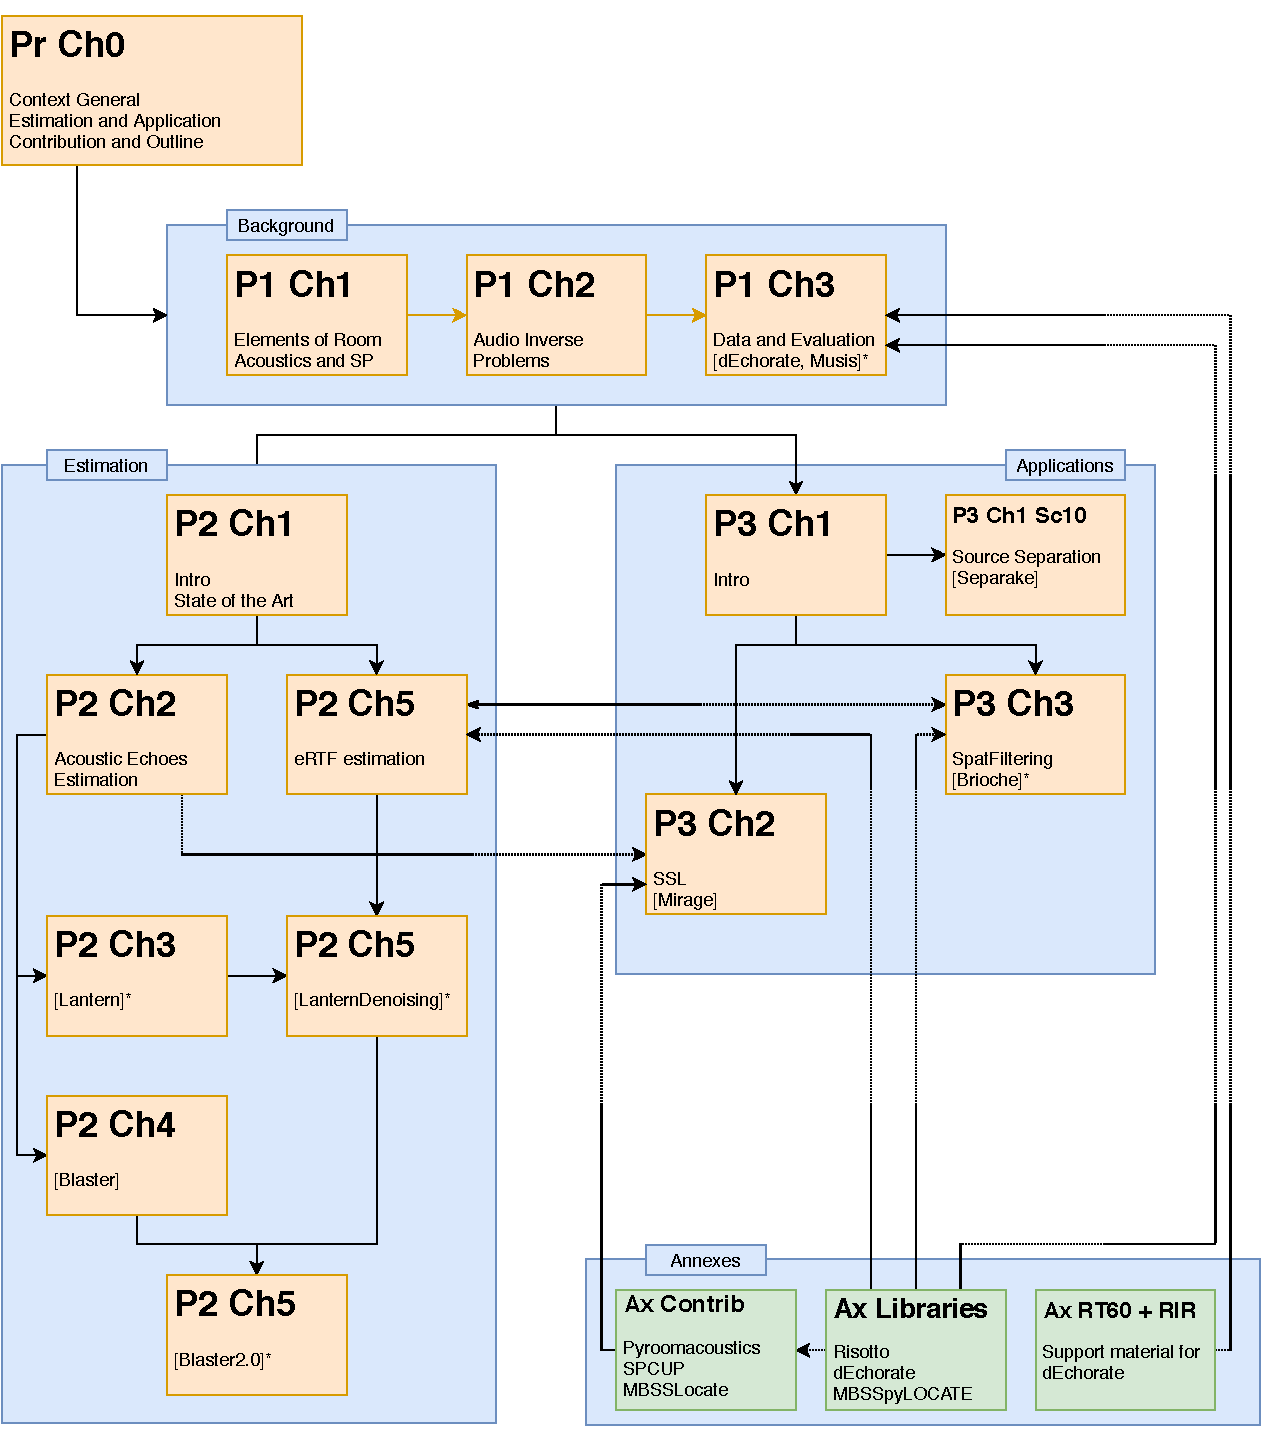
\includegraphics[width=\linewidth]{intro/thesis_mindmap.pdf}
    \end{sidecaption}
\end{figure}


\newthoughtpar{\cref{pt:background}\hspace{.3em}Room Acoustic meets Signal Processing}
\begin{description}
    \item[\cref{ch:acoustics}]\synopsisChAcoustics
    \item[\cref{ch:processing}]\synopsisChProcessing
\end{description}

\newthoughtpar{\cref{pt:estimation}\hspace{.3em}Acoustic Echoes Estimation}
This part focuses on how to estimate echoes from the only observation of microphone recordings.
\begin{description}
    \item[\cref{ch:estimation}]\synopsisChEstimation
    \item[\cref{ch:lantern}]\synopsisChLantern
    \item[\cref{ch:blaster}]\synopsisChBlaster
    \item[\cref{ch:dechorate}]\synopsisChDechorate
\end{description}


\newthoughtpar{\cref{pt:application}\hspace{.3em}Echo-aware Audio Scene Analysis}
In this part, we present some audio scene analysis problems that will be later discussed in their echo-aware extension.

\begin{description}
\item[\cref{ch:application}]\synopsisChApplication
\item[\cref{ch:separake}]\synopsisChSeparake
\item[\cref{ch:mirage}]\synopsisChMirage
\item[\cref{ch:dechorateapp}]\synopsisChDecharateApp
\end{description}

\newthought{Finally,} the dissertation concludes with~\cref{ch:conclusion}, which summarizes the contributions and raises several additional research questions.

\newpage
\section{List of contributions}
This dissertation draws heavily on the work and writing of the following papers, written jointly with several collaborators:

\begin{itemize}
    \item \fullcite{di2021dechorateB}
    \item \fullcite{di2020blasterB}
    \item \fullcite{di2019mirageB}
    \item \fullcite{deleforge2019audioB}
    \item \fullcite{lebarbenchon2018evaluationB}
    \item \fullcite{scheibler2018separakeB}
\end{itemize}

\newpage
\section{Don't panic!}
The reader will have already noticed that a large margin is left free on each manuscript page.
We will use it to insert personal comments, historical notes, additional insights, and figures and tables to complete each subject.
This graphic template is inspired by the work of \citeauthor{tufte1983visual}~\citeonly{tufte1983visual}\sidenote{
    The colophon of the thesis reports more information on the template.}
.
We emphasize the presence of clickable links by the \ExternalLink logo.
Code libraries are written in typewriter font, \eg/ \library{dEchorate}.

\subsection{Quick vademecum}
For the readers:
\begin{itemize}
    \item \textcolor{myorange}{orange} is used for clickable internal reference, such as for sections ~\cref{sec:intro:processing} and acronyms \acs{FFT};
    \item \textcolor{mygray}{grey} and \ExternalLink is used for clickable external link, such as \href{www.diegodicarlo.com}{my website\ExternalLink};
    \item reference sidenotes on the margin are used as footnotes, providing additional insights;
    \item italic sidenotes and figures without proper reference numbers on the margin are meant to provide optional information and can be read in a second moment;
    \item \textcolor{black!30}{\scriptsize\raisebox{1pt}{$\blacktriangleright$}}\hspace{0.2em}should capture the reader attention towards the important points;
    \item \textcolor{black!30}{\scriptsize\raisebox{1pt}{$\boldsymbol{?}$}}\hspace{0.2em}indicates a question-and-answer paragraph;
    \item \textcolor{black!30}{\scriptsize\raisebox{1pt}{$\rightleftarrows$}}\hspace{0.2em}indicates the presence of definitions by dichotomy;
    \item the following icon denotes the end of the chapter. \qed
\end{itemize}

\subsection{The golden ratio of the thesis}
This thesis has been written following personal stylistic rules:
\begin{itemize}
    \item after the the colon punctuation mark, ``:'', small caps. In case of list, items are delimited by semicolon punctuation mark ``;'';
    \item sidenotes number referring to a word superscripts the word itself, sidenotes referring to a whole sentence superscripts the corresponding full stop;
    \item N'ilazo color palette: black, grey and orange;
    \item at most three levels of sub-headings: section, subsection, and Tufte's \textit{new-thought}~\citeonly{tufte1983visual} to capture attention;
    \item the usage of dichotomies is privileged when presenting concepts and definitions, thus they are emphasized;
    \item each section should be introduced briefly at the end of the previous one to promote reading flow;
    \item no indentation, but well-separated text blocks;
\end{itemize}



% \newthought{Audio Signal Processing}
% \begin{itemize}
    %     \item Motivation
    %     \item Definitions, Function, Characteristics
%     \item Current challenges
% \end{itemize}

% \newthought{Inverse Problem}
% Starting with the effects to discover the causes has concerned physicists for centuries.

% While in many ways, mixtures are not different to any other audio signal, two research questions stand out prominently: • Can we obtain the sources sj from the mixture x? • Can we find the number of sources J from x? These two questions are addressed in the scientific fields of sound
% source separation and source count estimation


% Inverse problems appear when we want to see or examine something that we cannot access directly. What we have is an indirect measurement that contains hidden information.

% An inverse problem is always a counterpart of a direct problem, as shown in the schematic diagram below. The direct problem is going from object to data, and the inverse problem is about finding the object back from the data.

% The assumed few thousand taps. This model was very popular in the early stages of research [48]–[55]. Recently, interest has revived with sparse penalties which account for prior knowledge about the physical properties of AIRs, namely the facts that power concentrates in the direct path and the first early echoes [56]– [60] and that the time envelope decays exponentially [61], but these penalties have not yet been used in a BSS context.


% \section{Audio Inverse Problems}\label{sec:processing:inverse}
% \cite{kitic2015cosparse}
% \openepigraph{Their generality is of such a wide scope that onemayeven argue that solving inverse problems is what signal processing is all about}{Srdan Kiti\'c, \textit{Cosparse regularization of physics-driven inverse problems}}
% \openepigraph{everything is an optimization problem}{\citeonly{watson2001nonlinear}}
% \marginpar{
%     \footnotesize
%     One can see the paralelism with the engineering concepts: analysis and sythesis.
% }
% In~\cref{sec:intro:problem} we have informally defined \textit{inverse problems}, with an emphasis on inverse problems in signal processing.
% An inverse problem is a type of a mathematical problem where we start with the observations and we want to estimate model parameters that produced them.
% \\Inverse problems pervades all the field of science and engineering:
% source localization~\cite{},
% image processing~\cite{},
% acoustic imaging and tomography~\cite{},
% \marginpar{
%     \footnotesize
%     A historical example are the calculation of the Earth circunference by Eratosthenes in III century b.c.\\
%     and the calculations of Adams and Le Verrier which led to the discovery of Neptune from the perturbed trajectory of Uranus.
% }

% A inverse problems is defined as the counterpart of a \textit{forward}\sidenote{often referred to as \textit{direct}} problem.
% Without falling in and deep mathematical formalism and taxonomies which can be found in \citeonly{bal2012introduction},
% we will simply consider the following informal definition:
% \begin{center}
%     \textit{\emph{Forward problem} starts from known input, while \emph{inverse problem} starts from known output~\cite{santamarina2005discrete}.}
% \end{center}
% Both these problems focus on an operation relating maps objects of interest, called \textit{parameters} or \textit{variables},
% to information collected about these objects, called \textit{measurements}, \textit{data} or \textit{observation}.

% For instance, in our context, the direct problem may be the estimation of the \RIR/(s) starting from the known room parameters,
% and, the related inverse problem would be the estimation of such room properties from the observation of the \RIR/(s).

% Formally, a forward problem is defined through a mathematical model, described by a \textit{operation} $\scrM(\cdot)$
% mapping \textit{parameters} $x \in \scrX$ to the \textit{observation} (or measurement) $y \in \scrY$:
% \begin{equation}\label{eq:processing:model}
%     y = \scrM(x)
%     .
% \end{equation}
% Then, the inverse problem defines a method $\kinv{\scrM}$ that ``reverts'' $\scrM$ in order to recover (estimate) $x$ form the observation of $y$.
% % The operator $\scrM$ describes our best effort to construct a \textit{model} for the available data $y$.
% % The choice of $\scrX$ describes our best effort to characterize the space where we believe the parameters belong.

% As discussed in~\cite{bal2012introduction}, \textit{solving} the inverse problem consists in finding point(s) $x \in \scrX$ from (knowledge of) data $y \in \scrY$
% such that~\cref{eq:processing:model} or an approximation of~\cref{eq:processing:model} holds.
% Under this light, the operator $\scrM$ ant the choice of $\scrX$ describes our best effort to construct a \textit{model} for the data $y$ and
% the space where the parameters $x$ belong, respectively.
% \marginpar{
%     \footnotesize
%     one can already see the paralelism the the definition of the mixing process defined in~\cref{sec:intro:problem}
% }

% \textsc{For instance, in Case of} \textit{linear} inverse problem, and for $\scrY$ and $\scrX$ being vector spaces of dimensions $M$ and $N$ respectively,
% then the forward map can be written as a linear system:
% \begin{equation}\label{eq:processing:linear_forward}
%     \bfy = \bfM \bfx
% \end{equation}
% where $\bfM$ being a matrix, namely the operator $\scrM$ becomes a matrix multiplication by $M$.
% It follows that the inverse map associated to~\cref{eq:processing:linear_forward} is the application of the inverse matrix $\kinv{M}$.
% % While solving a direct problem the an operator needs to be found, in solving the inverse one either the operator is known and needs
% % to be $reverts$t

% Typically, forward problems are considered somehow the ``easier''.
% In fact, even in the observation model $\scrM$ is known perfectly, it is not always possible to find its counterpart.
% This because of
% \begin{itemize}
%     \item presence of \textit{noise} in the measurement which are not always additive and statistically independent \wrt/ $x$.
%     \item the problem is \textit{well-posed} and \textit{well-conditioned}, namely $\scrM$ needs be injective and stable.
%     In other words, some information is recoverable, other is completely lost, other highly sensible to noise
%     \sidenote{
%         \textbf{injective} ensure the uniqueness of the solution, while \textbf{stability}
%         ensure a continuity on the data.
%         These are known as the Hadamard's \textit{solvability conditions}.
%     }.
% \end{itemize}

% As we could images, many interesting and fundamental inverse problem are
% \textit{ill-posed} or \textit{ill-conditioned} in general, even in the following ``simple'' ones~\cite{kitic2015cosparse}:
% The solution to the deconvolution problem, where the direct inversion of the transfer function results in instabilities
% at high frequency; and the solution a linear system $\bfy = \bfM \bfx$ where $\bfM$ is invertible
% may lead to erroneous results and numerical instabilities.

% Therefore, sometimes ones have to settle for restring the set of solution $\scrC \subset \scrX$,
% where $\scrM$ is stable and injective\sidenote{This framework was originally proposed by Tikhonov.}.
% Promoting solution $x \in \scrC$ is can be achieved through \textit{model priors}, namely prior knowledge about solution, which can
% be classified in the following methodologies:
% the usage of \textit{geometric constraints} that deterministically define the solutions; the imposition of \textit{penalization}
% which ``promotes'' solution of a certain shape (\eg/ \textit{sparse}
% \sidenote{\textbf{sparsity} is a fundamental concept of this thesis, better discussed in~\cref{pt:estimation}
% } or \textit{smoothness});
% and casting the problem in a \textit{bayesian framework} which versatilely incorporate prior and posterior density function describing the data.

% Let us give two example of practical systems that will be recurrent thought out the entire thesis.

% \subsection{Selected Audio Inverse Problems}
% Here follow some famous problems in the field of audio signal processing with application to speech, music and environmental audio.
% Given the mixing process defined in~\cref{sec:processing:model},

% % \begin{description}
% %     \item[sound source separation and enhancements] as the problem of retrieving a (set of) source signal from a mixture.
% %     \item[sound source localization] estimation of source location from the observation of the sound production.
% %     This has sense as long as the impulse response convey space properties.
% %     \item[microphones calibration] estimation of the microphone placement.
% %     \item[\RIR/ estimation] estimation of the filters.
% %     Blind Channel Estimation or System Identification.
% %     \item[Acoustic Echoes Estimation] estimation of the filters
% %     \item[dereverberation] estimation of the filters
% %     \item[room geometry estimation] estimation of the room
% %     \item[automatich speech recognition]
% % \end{description}



%
% \newthought{Depending on the scenario}, all these problems exhibits strong inter-connections,
% namely the solution of one may be (dependent on) the solution of another.
% Therefore, exploiting expertise and knowledge,
% interconnect and hierarchical approaches may be built\sidenote{Machine Learing allows now for end2end approaches}:
% for instance, many spatial filtering techniques used for \SE/ rely on \SSL/ blocks;
% and in order to achieves \RooGE/, \AER/ must be done.
